\clearpage\subsection*{2−1 HTMLについて}
\refstepcounter{PagePtr}\label{P:HTML}
\refstepcounter{Exercise}
\subsection*{\theExercise HTMLの復習\label{E:HTML}}
{\bfseries
	考え方\newline

	第1回で作成した\ruby{自己紹介}{じこしょうかい}ページのタグや機能を理解することでHTMLについて自分の思ったとおりに作れるようになりましょう。}


\bigskip

HTMLは、タグという一つの機能をつかい、ウェブページを作り出します。\newline
タグというのは、{\textless}{\textgreater}{\textless}/{\textgreater}という形です。見覚えのある形ですね。\newline
例えば、

\ \ {\textless}p{\textgreater}文章をここに書きます。{\textless}/p{\textgreater}

のようなタグをpタグと\ruby{呼}{よ}びます。pタグはタグの間にある文章を表示します。\newline
まずは、第1回目の授業でみさなんが作成した自己紹介ページとその画像のファイルを第7回のフォルダにコピーし、それをmousepadでhtmlファイルを開いて見ましょう。

\begin{minipage}[b]{0.5\textwidth}
	\begin{enumerate}
		\begin{minipage}[b]{1.5\textwidth}
			\item \ \ cp \ \ {\textasciitilde}/01/self\_intro.html \ \ \ {\textasciitilde}/07/www/index.html\\
			\ \ cp \ \ {\textasciitilde}/01/face.png \ \ \ {\textasciitilde}/07/www/\\
			cpコマンドを使って、 自己紹介ページのhtmlと<img src="face.png" などimgタグで指定している画像ファイルを、 第7回のwwwディレクトリにコピーしましょう。"face.png"以外にも使っている画像ファイルがあればコピーしてください。\\
			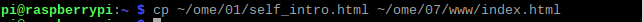
\includegraphics[width=14.73cm]{ome7-img033.png}
			\bigskip
		\end{minipage}

		\bigskip

		\item

		      \ \ cd \ \ {\textasciitilde}/07/www/\newline
		      cdコマンドを使って、(cpコマンドとは\ruby{違}{ちが}うよ。) 第7回のwwwディレクトリに\ruby{移動}{いどう}。


		\item \ \ mousepad\ \index.html

		      \ \ mousepadでコピーした自己紹介のhtmlを開いてみよう。

	\end{enumerate}
\end{minipage}
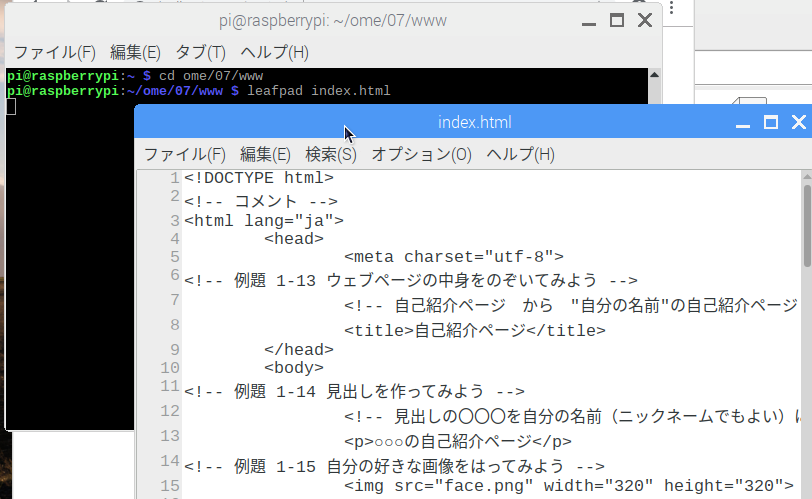
\includegraphics[width=0.45\textwidth]{ome7-img034.png}

\bigskip

開いたhtmlファイルの中に、実際にはウェブページに出てこない文章がちらほら見えます。

\ \ \ \ \ \ {\textless}!-{}- コメント -{}-{\textgreater}

それは、コメントという機能でウェブページには表示されない、メモのような機能でプログラムを書くときにあると便利です。HTMLに限らずHSPや様々なプログラム言語、はたまた現実世界でもメモというのは大切なので必要な情報はしっかりと書いておきましょう。

self\_intro.html内に使われたタグをまとめました。これを参考に自己紹介ページをより良くしていきましょう。

\clearpage
HTMLまとめ\ \

\begin{center}
	\tablefirsthead{}
	\tablehead{}
	\tabletail{}
	\tablelasttail{}
	\begin{supertabular}{|m{4.0cm}|m{12.0cm}|}
		\hline
		タグ名 &

		\ruby{効果}{こうか}\\\hline

		{\textless}title{\textgreater}{\textless}/title{\textgreater} &
		ウェブページのタイトルをつける\\\hline
		{\textless}h1{\textgreater}{\textless}/h1{\textgreater} &
		見出し(h1~h6)まで使える。h1が一番大きい\\\hline
		{\textless}ul{\textgreater}{\textless}/ul{\textgreater} &

		点付のリスト。リストの\ruby{項目}{こうもく}はliを使って表す\\\hline
		{\textless}li{\textgreater}{\textless}/li{\textgreater} &
		リストの項目。ulもしくはolタグなどの中で使う\\\hline
		{\textless}p{\textgreater}{\textless}/p{\textgreater} &
		\ruby{段落}{だんらく}を作るために使う。文字を表示したいときはこれを使う。改行は自動で行われるので自分のタイミングで行いたいときは{\textless}br{\textgreater}を使う\\\hline
		{\textless}br{\textgreater} &
		改行. pの中でも使うことができる\\\hline
		{\textless}i{\textgreater}{\textless}/i{\textgreater} &
		イタリック(少し\ruby{傾}{かたむ}いた感じの文字)\\\hline
		{\textless}u{\textgreater}{\textless}/u{\textgreater} &
		文字の下に線を引くときに使う\\\hline
		{\textless}a href=””{\textgreater}{\textless}/a{\textgreater} &
		リンクを貼りたいときに使う。hrefにはクリックしたときに飛びたいURLを入れる。\\\hline
		{\textless}img src=””{\textgreater} &
		画像を表示するときに使用する。srcには画像の場所を指定する。ラズベリーパイの中の画像を指定しても、URLとして指定しても良い。\\\hline
		{\textless}ol{\textgreater}{\textless}/ol{\textgreater} &
		番号付きのリスト.
		liでリストの項目を決める。

		番号はliの書いた順番通りになる\\\hline
	\end{supertabular}
\end{center}

\bigskip

HTMLで使いたい色を探すときにはここを使うと便利です。

\url{https://www.colordic.org/m/}\newline
地下鉄のシンボルカラーとカラーコードで使いたい色がわかるはずです。

\url{https://www.colordic.org/}\newline
色の名前とカラーコードがわかります。色がまんべんなくあります。

\url{https://tech-unlimited.com/color.html}\newline
上級者向け、色の三原色というものから実際にHTML用のカラーコードに変えるサイトです。

\clearpage
また、HTMLにはボタンや文字を書き込む部分も作れます。\newline
通常見るだけのウェブページだったものがデータの送受信を可能とするなど、可能性を広げられます。

一部のタグを下に\ruby{記載}{きさい}します。

\begin{center}
	\tablefirsthead{}
	\tablehead{}
	\tabletail{}
	\tablelasttail{}
	\begin{supertabular}{|m{8.6cm}|m{7.91cm}|}
		\hline
		{\textless}form{\textgreater}{\textless}/form{\textgreater}

		(使用例)

		\ {\textless}form action=”cgi-bin/formmail.cgi” {\textgreater} &
		入力送信フォームを作成

		formタグの中に
		{\textless}input{\textgreater},
		{\textless}select{\textgreater},
		{\textless}textarea{\textgreater}
		などをいれることで

		ボタンや文字入力欄を作れる\\\hline
		{\textless}input{\textgreater}{\textless}/input{\textgreater}

		(使用例)

		{\textless}input type=”password” name=”pass”{\textgreater} &
		文字の入力や、ボタンなどを作成するタグ。


		inputの次にtypeなどの\ruby{属性}{ぞくせい}を入れることで一行の文章やパスワードの入力などを決定する\\\hline
	\end{supertabular}
\end{center}

\bigskip

それでは、formを使った例題を説いてみましょう。

例題\newline
自己紹介ページの一番下から2行上あたりにある{\textless}/body{\textgreater}の上の行から{\textless}form{\textgreater}タグで文字の入力をし、送信ボタンを\ruby{押}{お}せる機能を書きましょう。

考え方\newline
はじめに、formタグの間({\textless}form{\textgreater}
**ここ**{\textless}/form{\textgreater})に、inputタグでテキストボックスを作る。そして、同じようにinputタグを使って送信ボタンという名前のボタンを作成する。

1.{\textless}form{\textgreater}{\textless}/form{\textgreater}を書き込めるスペースを作ろう。



\centering
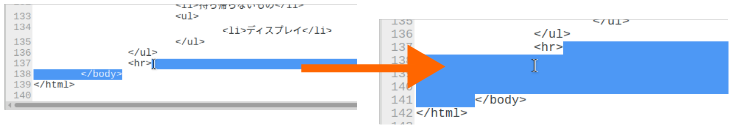
\includegraphics[width=\textwidth]{ome7-img035.png}
\flushleft

2.{\textless}form{\textgreater}タグを書き足そう。



\centering
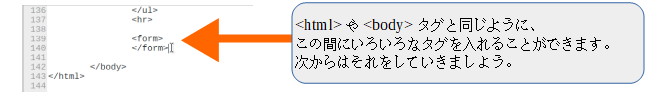
\includegraphics[width=\textwidth]{ome7-img036.png}
\flushleft


\bigskip


\bigskip

3.{\textless}form{\textgreater}タグの間に、行を作り「テキストボックス」という文字が出るようにしよう。\newline
\ \ {\textless}form{\textgreater}\newline
\ \ \ \ \textbf{\textit{{\textless}p{\textgreater}テキストボックス{\textless}/p{\textgreater}}}\newline
\ \ {\textless}/form{\textgreater}

\bigskip

\clearpage

4.次の行に{\textless}input{\textgreater}タグを入れよう。その際に、テキストを書き込めるようにしよう。

%\newline
\ \ 画像のようにするためには、\newline
\ \ {\textless}form{\textgreater}\newline
\ \ \ \ {\textless}p{\textgreater}テキストボックス{\textless}/p{\textgreater}\newline
\ \ \ \ \textbf{\textit{{\textless}input \ \ type=”text” \ \ size=”10”{\textgreater}}}\newline
\ \ {\textless}/form{\textgreater}

\centering
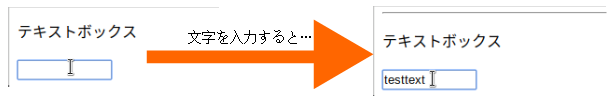
\includegraphics[width=16.3cm]{ome7-img037.png}
\flushleft

5.同じようなやり方で、先にかいた{\textless}input{\textgreater}タグから改行して次の行に{\textless}input{\textgreater}タグで送信ボタンを作成しよう。\newline
\ \ \ \ \textbf{\textit{{\textless}input type=”submit” value=”送信”{\textgreater}}}

6.作成したHTMLファイルを保存し、実際にブラウザで作成されているか確認してみましょう。\newline


このように、formタグ、inputタグには便利な機能があります。\newline
以下に、inputタグの属性を一部記載しておきますので、\textbf{参考にして}問題を解いていきましょう。


\bigskip

\clearpage
\refstepcounter{Question}\theQuestion\label{Q:HTML}\newline
\begin{enumerate}
	\item 最初に書いたテキストボックスの属性をパスワード入力ボックスに書き換えてみよう。
	\item 食べ物の名前を{\textless}p{\textgreater}タグを使って3つ追加してその横にチェックボックスを置きましょう。
	\item リセットボタンを送信ボタンの次の行に追加してみよう。
\end{enumerate}

\samepage

わからなかったら、先生に質問をすること。その間は\ruby{一覧}{いちらん}を見て考えてみよう。

inputタグの機能になるもの

\begin{flushleft}
	\tablefirsthead{}
	\tablehead{}
	\tabletail{}
	\tablelasttail{}
	\begin{supertabular}{|m{3.4459999cm}|m{7.9160004cm}|}
		\hline
		type=”text” &
		1行のテキストボックスを作ります。\newline
		sizeの属性を指定することで大きさも決定できる。\\\hline
		type=”password” &
		パスワード用のテキストボックスを作ります。\newline

		入力されたら*のマークなどに置き換わります。送信する際には\ruby{普通}{ふつう}の文字で送られるのに注意。\\\hline
		type=”checkbox” &
		チェックボックスを作ります。
		複数\ruby{選択}{せんたく}可能で、checked属性を指定すると予めチェックが入ったかどうかを決めれる。\\\hline
		type=”radio” &
		ラジオボタンを作ります。
		複数の中から1つしか選択できないのが\ruby{特徴}{とくちょう}。\newline
		こちらもcheckedで\ruby{状態}{じょうたい}を決めれる。\\\hline
		type=”submit” &
		送信ボタンを作ります。\\\hline
		type=”button” &
		普通のボタンを作ります。\\\hline
		type=”image” &
		画像のボタンを作ります。\newline
		使用する画像ファイルは、src属性で指定しましょう。またalt属性が\ruby{必須}{ひっす}。\\\hline
		type=”reset” &
		リセットボタンを作ります。

		このボタンを押すと、書いていたデータがなくなり最初の状態に\ruby{戻}{もど}ります。\\\hline
	\end{supertabular}
\end{flushleft}

\bigskip

\clearpage
\refstepcounter{PagePtr}\label{P:HP}
\refstepcounter{Exercise}
\subsection*{2−2 \theExercise 自分のホームページを公開しよう\label{E:myHP}}
考え方


クライアントとサーバーと呼ばれるコンピュータがあります。クライアントとはサービスを利用するコンピュータです。サーバーとはそれと\ruby{逆}{ぎゃく}にサービスを提供しているコンピュータです。クライアントとサーバーは同じコンピュータにあっても
OK です。例えば、Googleは検索するためのウェブサイトを提供しています。ウェブサイトを提供するサーバーをウェブサーバーと呼びます。自分のホームページを公開するためには、ウェブサーバーを動かす必要があります。

注意

今回のみんなのホームページはローカルIPの間だけです。つまり、インターネット上に公開はしません。これを公開して、実際確認したりみんなで見せ合いをしてみましょう。


\bigskip

1.まず
{\textasciitilde}/07/wwwのディレクトリに移りましょう。

\ \ ターミナルを立ち上げて次のコマンドを打ちましょう。

\ \ cd {\textasciitilde}/07/www


\bigskip

2.サーバーを動かしてみましょう。

\ \ 次のコマンドを打ちましょう。

\ \  ./webserver.py

\ \ を実行するとウェブサーバが動き始めます。

\ \ webserver.pyを起動したディレクトリがドキュメントルートになります。

\ \ これはファイルシステムのルートディレクトリとは別のものでドキュメントルートはウェブ

\ \ サーバから見たルートディレクトリのことです。

\ \ つまりウェブサーバーしかそのディレクトリをルートディレクトリとは認識しません。

\ \ ディレクトリに関しては第3回の教科書3.3.2 「ディレクトリの関係」を参考にしてください。


\centering
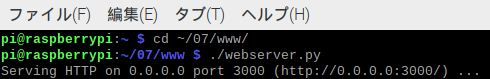
\includegraphics[width=0.73\textwidth]{ome7-img038.png}
\flushleft

3.サーバーが動いているかどうかを確認してみましょう。

\ \ 別のターミナルを立ち上げ、次のコマンドを打ちましょう。

\ \  nmap localhost

\ \ 今回使っているポート番号は:3000です。STATE(状態)がopen(開く)になっています。

\ \ これでサーバーが動いていることが分かります。

\centering
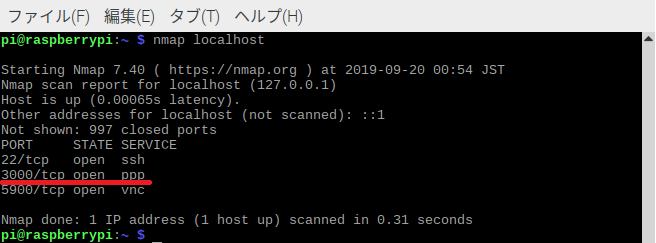
\includegraphics[width=0.75\textwidth]{ome7-img039.png}
\flushleft

\clearpage


4.みなさんが作ったウェブページを表示してみましょう。

\ \ みなさんが作ったindex.htmlの場所はwebserver.pyを起動したディレクトリと同じでしたね。「2」で説明したドキュメントルートです。

\ \ これはwebserver.pyを起動したディレクトリ

\ \  {\textasciitilde}/07/www/

\ \ を指しています。


\bigskip

\ \ 次にブラウザのアドレスバーに打つURLはどのように書けばいいのでしょうか。

\ \ URLの書き方は次のようになります。

\ \ なので自分のパソコンのサーバーを見るには

\centering

\includegraphics[width=13.894cm]{ome7-img040.png}
\flushleft

\ \  \url{http://localhost:3000/}

\ \ というURLになります。

\ \ サーバー名の後の/(スラッシュ)はドキュメントルートを示しています。

\ \ ブラウザはファイル名を指定しないとindex.htmlというファイルを開くように\ruby{設定}{せってい}されて\ \ います。

\ \  \url{http://localhost:3000/}

\ \ をブラウザのアドレスバーに打ってみましょう。

\ \ みなさんが作ったウェブページのHTMLが表示されましたね。

\ \ これは

\ \  \url{http://localhost:3000/index.html}

\ \ と入力しているのと同じことです。

\bigskip

\centering
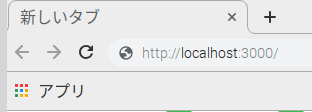
\includegraphics[width=9.551cm]{ome7-img041.png}
\flushleft


\bigskip


\bigskip


\refstepcounter{Exercise}
\clearpage\subsection*{2−3 \theExercise 友だちのホームページを見てみよう}
\addtocounter{Exercise}{-1}\refstepcounter{Exercise}\label{friend}


\centering
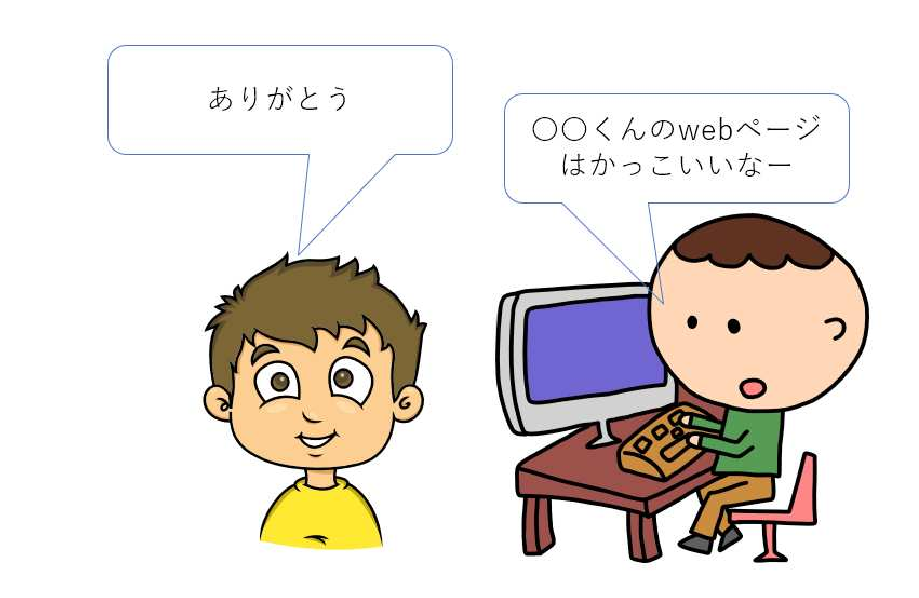
\includegraphics[width=10.423cm]{ome7-img042}
\flushleft


\bigskip



1.
\ruby{左隣}{ひだりどなり}の友達のIPアドレスを確認しよう。

\ \ 友達のターミナルで次のコマンドをうってもらいましょう。

\ \ hostname -I

\ \ そのIPアドレスをメモしましょう。

\ \ [\underline{    }さんのIP:\underline{              }]


\bigskip

2.友達のウェブページを見て見ましょう。

\ \ 自分のサーバーを見るときは

\ \  \url{http://localhost:3000/}

\ \ でした。localhostというのが自分のサーバーという意味でした。

\ \ 今回は友達のサーバーを見たいのでlocalhostの代わりに友達のIPアドレスを打ちましょう。

\ \  \url{http://xxx.xxx.xxx.xxx:3000/}

\ \ \  \url{http://xxx.xxx.xxx.xxx:3000/index.html}

\ \ をブラウザのアドレスバーに打ってみましょう。

\ \ もし左隣の友達のIPアドレスが192.162.33.5だったら

\ \  \url{http://192.162.33.5:3000/index.html}

\ \ となります。

\ \ 友達のウェブページが表示されたら成功です!


\bigskip


\centering
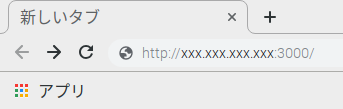
\includegraphics[width=10.659cm]{ome7-img043.png}
\flushleft

\clearpage\subsection*{\bfseries
	注意}

	\ref{friend}の友達のホームページを見てみようでは、以下の図のように同じルータにつながっているラズベリーパイが公開しているホームページは、見ることができます。\ruby{基本}{きほん}同じグループの子たちのホームページは見れるので確認してみてください。

\centering
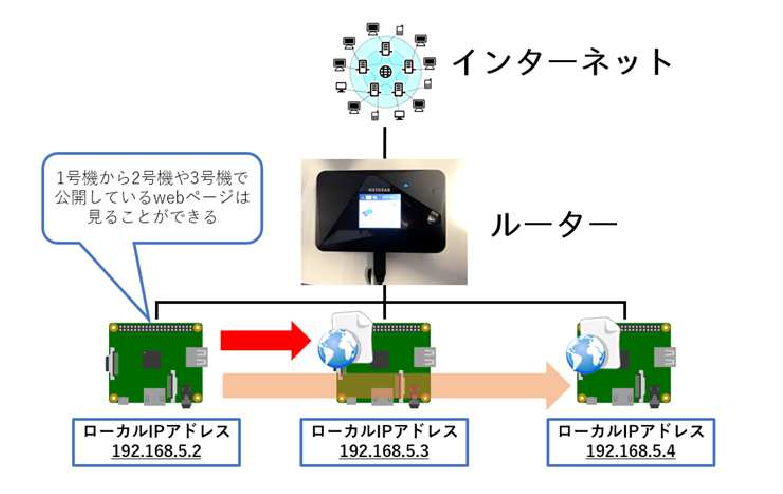
\includegraphics[width=0.75\textwidth]{ome7-img044}
\flushleft


\bigskip



あと、他のルータに接続しているラズベリーパイが公開しているホームページは今回みることができません。実際に試してみても面白いと思います。


\bigskip

\centering
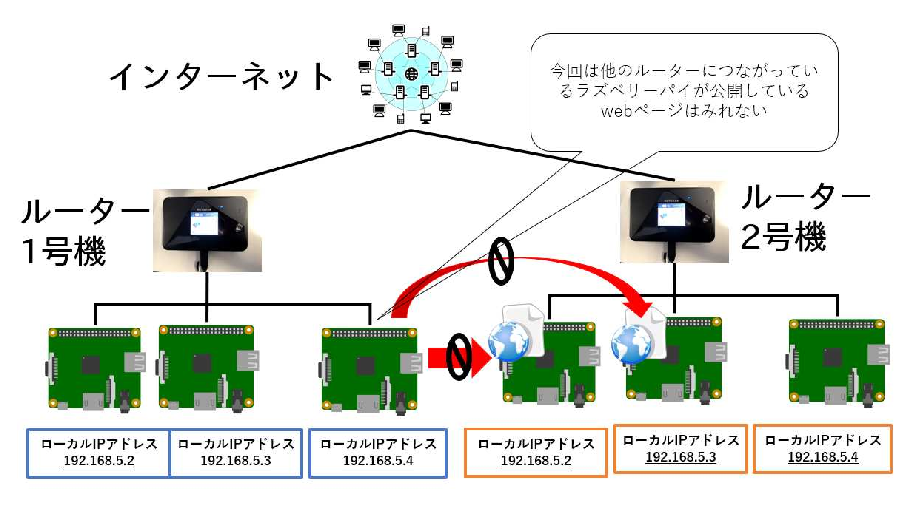
\includegraphics[width=0.75\textwidth]{ome7-img045}
\flushleft


\bigskip

\refstepcounter{Question}\theQuestion 他のグループの友達のホームページを見てみよう、自分とは違うWi-Fiルータに接続している友達のホームページは見れたかどうか答えに書こう\label{Q:otherHP}



{\bfseries
	\addBlank{答え}}


\bigskip

\if0


	参考 接続できるネットワーク(Wi-Fiルータ)

	NTGR-4643\ \ \ \ パスワード 33995460

	NTGR-3EBC\ \ \ \ パスワード 34986626

	NTGR-3DFC\ \ \ \ パスワード 36976828

\fi

\bigskip


\bigskip
